\documentclass{standalone}
\usepackage{tikz}
\usetikzlibrary{patterns, positioning}


\begin{document}
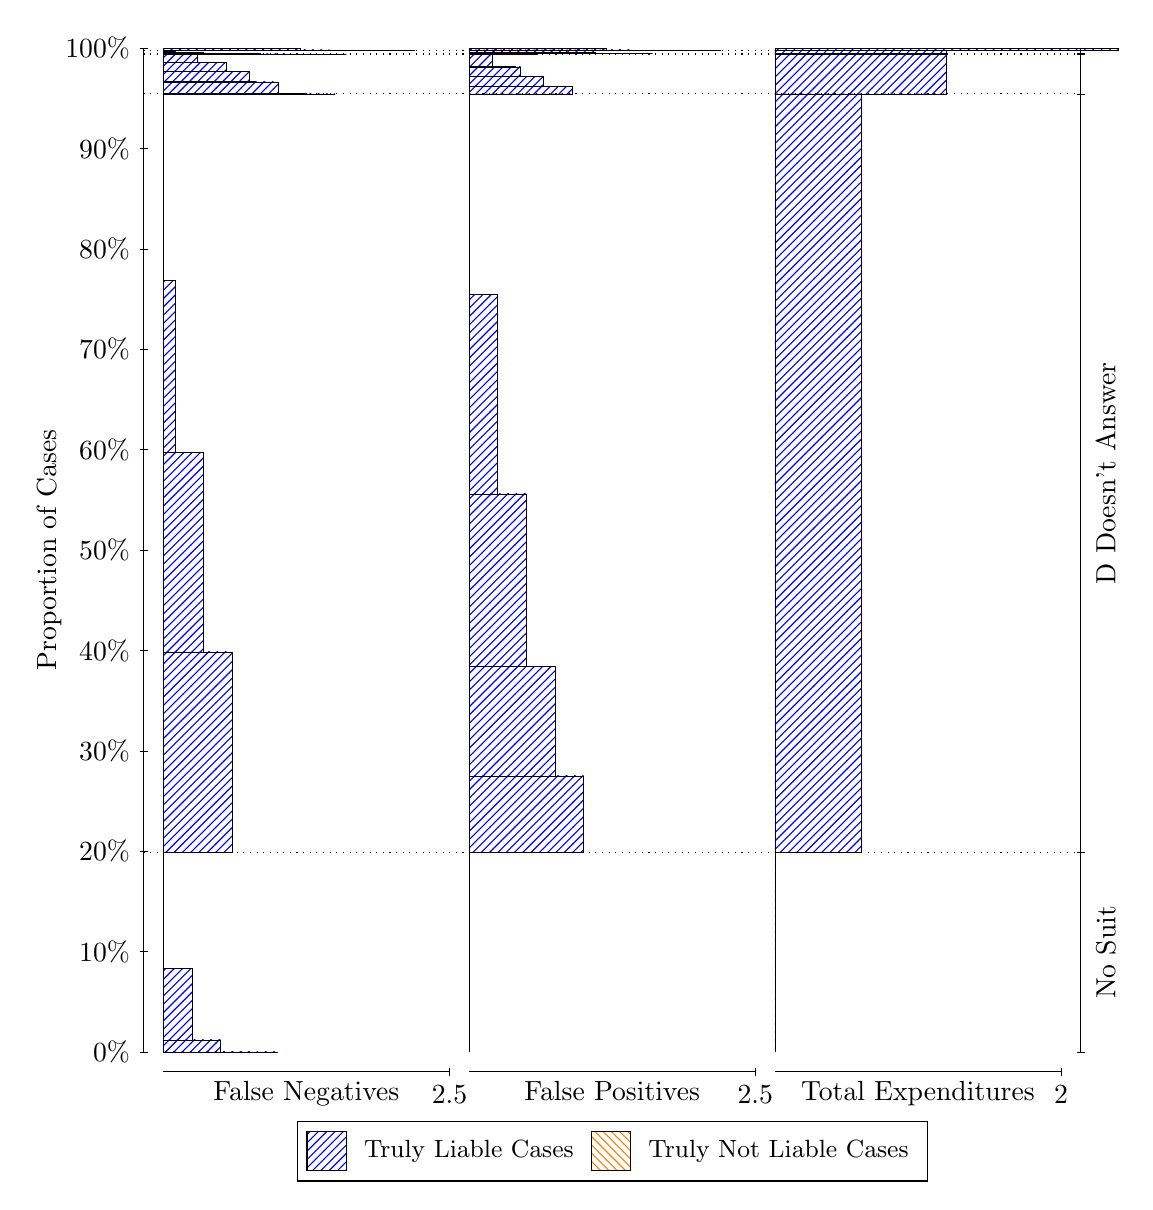
\begin{tikzpicture}
\draw[black, very thin] (1.5,1.75) -- (1.5,14.5);
\node[rotate=90, text=black, anchor=center] at (0.3, 8.125) {Proportion of Cases};
\draw[black, very thin] (1.45,1.75) -- (1.55,1.75);
\node[text=black, anchor=east] at (1.45, 1.75) {0\%};
\draw[black, very thin] (1.45,3.025) -- (1.55,3.025);
\node[text=black, anchor=east] at (1.45, 3.025) {10\%};
\draw[black, very thin] (1.45,4.3) -- (1.55,4.3);
\node[text=black, anchor=east] at (1.45, 4.3) {20\%};
\draw[black, very thin] (1.45,5.575) -- (1.55,5.575);
\node[text=black, anchor=east] at (1.45, 5.575) {30\%};
\draw[black, very thin] (1.45,6.85) -- (1.55,6.85);
\node[text=black, anchor=east] at (1.45, 6.85) {40\%};
\draw[black, very thin] (1.45,8.125) -- (1.55,8.125);
\node[text=black, anchor=east] at (1.45, 8.125) {50\%};
\draw[black, very thin] (1.45,9.4) -- (1.55,9.4);
\node[text=black, anchor=east] at (1.45, 9.4) {60\%};
\draw[black, very thin] (1.45,10.675) -- (1.55,10.675);
\node[text=black, anchor=east] at (1.45, 10.675) {70\%};
\draw[black, very thin] (1.45,11.95) -- (1.55,11.95);
\node[text=black, anchor=east] at (1.45, 11.95) {80\%};
\draw[black, very thin] (1.45,13.225) -- (1.55,13.225);
\node[text=black, anchor=east] at (1.45, 13.225) {90\%};
\draw[black, very thin] (1.45,14.5) -- (1.55,14.5);
\node[text=black, anchor=east] at (1.45, 14.5) {100\%};

\draw[black, very thin] (13.4,1.75) -- (13.4,14.5);
\draw[black, very thin] (13.35,1.75) -- (13.45,1.75);
\node[anchor=west] at (13.35, 1.75) {};
\draw[black, very thin] (13.35,4.2806) -- (13.45,4.2806);
\node[anchor=west] at (13.35, 4.2806) {};
\draw[black, very thin] (13.35,13.917) -- (13.45,13.917);
\node[anchor=west] at (13.35, 13.917) {};
\draw[black, very thin] (13.35,14.419) -- (13.45,14.419);
\node[anchor=west] at (13.35, 14.419) {};
\draw[black, very thin] (13.35,14.43) -- (13.45,14.43);
\node[anchor=west] at (13.35, 14.43) {};
\draw[black, very thin] (13.35,14.467) -- (13.45,14.467);
\node[anchor=west] at (13.35, 14.467) {};
\draw[black, very thin] (13.35,14.5) -- (13.45,14.5);
\node[anchor=west] at (13.35, 14.5) {};

\draw[black, very thin, pattern color=blue, pattern=north east lines] (1.75,1.75) rectangle (3.2033,1.75);
\draw[black, very thin, pattern color=blue, pattern=north east lines] (1.75,1.75) rectangle (2.84,1.7513);
\draw[black, very thin, pattern color=blue, pattern=north east lines] (1.75,1.7513) rectangle (2.4767,1.9039);
\draw[black, very thin, pattern color=blue, pattern=north east lines] (1.75,1.9039) rectangle (2.1133,2.8086);
\draw[black, very thin, pattern color=orange, pattern=north west lines] (1.75,2.8086) rectangle (1.75,2.8086);
\draw[black, very thin, pattern color=blue, pattern=north east lines] (1.75,2.8086) rectangle (1.75,4.2806);
\draw[black, very thin, pattern color=blue, pattern=north east lines] (1.75,4.2806) rectangle (2.622,6.8304);
\draw[black, very thin, pattern color=blue, pattern=north east lines] (1.75,6.8304) rectangle (2.2587,9.36);
\draw[black, very thin, pattern color=blue, pattern=north east lines] (1.75,9.36) rectangle (1.8953,11.553);
\draw[black, very thin, pattern color=orange, pattern=north west lines] (1.75,11.553) rectangle (1.75,11.553);
\draw[black, very thin, pattern color=blue, pattern=north east lines] (1.75,11.553) rectangle (1.75,13.917);
\draw[black, very thin, pattern color=blue, pattern=north east lines] (1.75,13.917) rectangle (3.93,13.917);
\draw[black, very thin, pattern color=blue, pattern=north east lines] (1.75,13.917) rectangle (3.6393,13.917);
\draw[black, very thin, pattern color=blue, pattern=north east lines] (1.75,13.917) rectangle (3.5667,13.92);
\draw[black, very thin, pattern color=blue, pattern=north east lines] (1.75,13.92) rectangle (3.276,13.92);
\draw[black, very thin, pattern color=blue, pattern=north east lines] (1.75,13.92) rectangle (3.2033,14.069);
\draw[black, very thin, pattern color=blue, pattern=north east lines] (1.75,14.069) rectangle (2.9127,14.076);
\draw[black, very thin, pattern color=blue, pattern=north east lines] (1.75,14.076) rectangle (2.84,14.2);
\draw[black, very thin, pattern color=blue, pattern=north east lines] (1.75,14.2) rectangle (2.5493,14.317);
\draw[black, very thin, pattern color=blue, pattern=north east lines] (1.75,14.317) rectangle (2.4767,14.319);
\draw[black, very thin, pattern color=blue, pattern=north east lines] (1.75,14.319) rectangle (2.186,14.419);
\draw[black, very thin, pattern color=orange, pattern=north west lines] (1.75,14.419) rectangle (1.75,14.419);
\draw[black, very thin, pattern color=blue, pattern=north east lines] (1.75,14.419) rectangle (4.0753,14.419);
\draw[black, very thin, pattern color=blue, pattern=north east lines] (1.75,14.419) rectangle (3.712,14.419);
\draw[black, very thin, pattern color=blue, pattern=north east lines] (1.75,14.419) rectangle (3.3487,14.425);
\draw[black, very thin, pattern color=blue, pattern=north east lines] (1.75,14.425) rectangle (2.9853,14.43);
\draw[black, very thin, pattern color=blue, pattern=north east lines] (1.75,14.43) rectangle (2.622,14.43);
\draw[black, very thin, pattern color=orange, pattern=north west lines] (1.75,14.43) rectangle (1.75,14.43);
\draw[black, very thin, pattern color=blue, pattern=north east lines] (1.75,14.43) rectangle (2.622,14.43);
\draw[black, very thin, pattern color=blue, pattern=north east lines] (1.75,14.43) rectangle (2.2587,14.446);
\draw[black, very thin, pattern color=blue, pattern=north east lines] (1.75,14.446) rectangle (1.8953,14.464);
\draw[black, very thin, pattern color=orange, pattern=north west lines] (1.75,14.464) rectangle (1.75,14.464);
\draw[black, very thin, pattern color=blue, pattern=north east lines] (1.75,14.464) rectangle (1.75,14.467);
\draw[black, very thin, pattern color=blue, pattern=north east lines] (1.75,14.467) rectangle (4.9473,14.467);
\draw[black, very thin, pattern color=blue, pattern=north east lines] (1.75,14.467) rectangle (4.584,14.467);
\draw[black, very thin, pattern color=blue, pattern=north east lines] (1.75,14.467) rectangle (4.2207,14.467);
\draw[black, very thin, pattern color=blue, pattern=north east lines] (1.75,14.467) rectangle (3.8573,14.475);
\draw[black, very thin, pattern color=blue, pattern=north east lines] (1.75,14.475) rectangle (3.494,14.492);
\draw[black, very thin, pattern color=blue, pattern=north east lines] (1.75,14.492) rectangle (3.1307,14.499);
\draw[black, very thin, pattern color=blue, pattern=north east lines] (1.75,14.499) rectangle (2.7673,14.5);
\draw[black, very thin, pattern color=blue, pattern=north east lines] (1.75,14.5) rectangle (2.404,14.5);
\draw[black, very thin, pattern color=blue, pattern=north east lines] (1.75,14.5) rectangle (2.0407,14.5);
\draw[black, very thin, pattern color=orange, pattern=north west lines] (1.75,14.5) rectangle (1.75,14.5);
\draw[black, very thin, pattern color=orange, pattern=north west lines] (5.6333,1.75) rectangle (5.6333,1.75);
\draw[black, very thin, pattern color=blue, pattern=north east lines] (5.6333,1.75) rectangle (5.6333,4.2806);
\draw[black, very thin, pattern color=orange, pattern=north west lines] (5.6333,4.2806) rectangle (7.0867,4.2806);
\draw[black, very thin, pattern color=blue, pattern=north east lines] (5.6333,4.2806) rectangle (7.0867,5.257);
\draw[black, very thin, pattern color=blue, pattern=north east lines] (5.6333,5.257) rectangle (6.7233,6.6451);
\draw[black, very thin, pattern color=blue, pattern=north east lines] (5.6333,6.6451) rectangle (6.36,8.838);
\draw[black, very thin, pattern color=blue, pattern=north east lines] (5.6333,8.838) rectangle (5.9967,11.368);
\draw[black, very thin, pattern color=blue, pattern=north east lines] (5.6333,11.368) rectangle (5.6333,13.917);
\draw[black, very thin, pattern color=orange, pattern=north west lines] (5.6333,13.917) rectangle (6.9413,13.917);
\draw[black, very thin, pattern color=blue, pattern=north east lines] (5.6333,13.917) rectangle (6.9413,14.017);
\draw[black, very thin, pattern color=orange, pattern=north west lines] (5.6333,14.017) rectangle (6.6507,14.017);
\draw[black, very thin, pattern color=blue, pattern=north east lines] (5.6333,14.017) rectangle (6.6507,14.019);
\draw[black, very thin, pattern color=blue, pattern=north east lines] (5.6333,14.019) rectangle (6.578,14.136);
\draw[black, very thin, pattern color=blue, pattern=north east lines] (5.6333,14.136) rectangle (6.2873,14.26);
\draw[black, very thin, pattern color=blue, pattern=north east lines] (5.6333,14.26) rectangle (6.2147,14.267);
\draw[black, very thin, pattern color=blue, pattern=north east lines] (5.6333,14.267) rectangle (5.924,14.416);
\draw[black, very thin, pattern color=blue, pattern=north east lines] (5.6333,14.416) rectangle (5.8513,14.416);
\draw[black, very thin, pattern color=blue, pattern=north east lines] (5.6333,14.416) rectangle (5.6333,14.419);
\draw[black, very thin, pattern color=orange, pattern=north west lines] (5.6333,14.419) rectangle (6.5053,14.419);
\draw[black, very thin, pattern color=blue, pattern=north east lines] (5.6333,14.419) rectangle (6.5053,14.419);
\draw[black, very thin, pattern color=blue, pattern=north east lines] (5.6333,14.419) rectangle (6.142,14.424);
\draw[black, very thin, pattern color=blue, pattern=north east lines] (5.6333,14.424) rectangle (5.7787,14.43);
\draw[black, very thin, pattern color=blue, pattern=north east lines] (5.6333,14.43) rectangle (5.6333,14.43);
\draw[black, very thin, pattern color=orange, pattern=north west lines] (5.6333,14.43) rectangle (7.9587,14.43);
\draw[black, very thin, pattern color=blue, pattern=north east lines] (5.6333,14.43) rectangle (7.9587,14.43);
\draw[black, very thin, pattern color=blue, pattern=north east lines] (5.6333,14.43) rectangle (7.5953,14.433);
\draw[black, very thin, pattern color=blue, pattern=north east lines] (5.6333,14.433) rectangle (7.232,14.452);
\draw[black, very thin, pattern color=blue, pattern=north east lines] (5.6333,14.452) rectangle (6.8687,14.467);
\draw[black, very thin, pattern color=blue, pattern=north east lines] (5.6333,14.467) rectangle (6.5053,14.467);
\draw[black, very thin, pattern color=orange, pattern=north west lines] (5.6333,14.467) rectangle (8.8307,14.467);
\draw[black, very thin, pattern color=blue, pattern=north east lines] (5.6333,14.467) rectangle (8.8307,14.467);
\draw[black, very thin, pattern color=blue, pattern=north east lines] (5.6333,14.467) rectangle (8.4673,14.467);
\draw[black, very thin, pattern color=orange, pattern=north west lines] (5.6333,14.467) rectangle (8.4673,14.467);
\draw[black, very thin, pattern color=blue, pattern=north east lines] (5.6333,14.467) rectangle (8.4673,14.467);
\draw[black, very thin, pattern color=blue, pattern=north east lines] (5.6333,14.467) rectangle (8.104,14.467);
\draw[black, very thin, pattern color=orange, pattern=north west lines] (5.6333,14.467) rectangle (8.104,14.467);
\draw[black, very thin, pattern color=blue, pattern=north east lines] (5.6333,14.467) rectangle (8.104,14.468);
\draw[black, very thin, pattern color=blue, pattern=north east lines] (5.6333,14.468) rectangle (7.7407,14.468);
\draw[black, very thin, pattern color=orange, pattern=north west lines] (5.6333,14.468) rectangle (7.7407,14.468);
\draw[black, very thin, pattern color=blue, pattern=north east lines] (5.6333,14.468) rectangle (7.7407,14.475);
\draw[black, very thin, pattern color=blue, pattern=north east lines] (5.6333,14.475) rectangle (7.3773,14.475);
\draw[black, very thin, pattern color=orange, pattern=north west lines] (5.6333,14.475) rectangle (7.3773,14.475);
\draw[black, very thin, pattern color=blue, pattern=north east lines] (5.6333,14.475) rectangle (7.3773,14.492);
\draw[black, very thin, pattern color=blue, pattern=north east lines] (5.6333,14.492) rectangle (7.014,14.499);
\draw[black, very thin, pattern color=blue, pattern=north east lines] (5.6333,14.499) rectangle (6.6507,14.5);
\draw[black, very thin, pattern color=blue, pattern=north east lines] (5.6333,14.5) rectangle (6.2873,14.5);
\draw[black, very thin, pattern color=blue, pattern=north east lines] (5.6333,14.5) rectangle (5.924,14.5);
\draw[black, very thin, pattern color=orange, pattern=north west lines] (9.5167,1.75) rectangle (9.5167,1.75);
\draw[black, very thin, pattern color=blue, pattern=north east lines] (9.5167,1.75) rectangle (9.5167,4.2806);
\draw[black, very thin, pattern color=orange, pattern=north west lines] (9.5167,4.2806) rectangle (10.607,4.2806);
\draw[black, very thin, pattern color=blue, pattern=north east lines] (9.5167,4.2806) rectangle (10.607,13.917);
\draw[black, very thin, pattern color=orange, pattern=north west lines] (9.5167,13.917) rectangle (11.697,13.917);
\draw[black, very thin, pattern color=blue, pattern=north east lines] (9.5167,13.917) rectangle (11.697,14.419);
\draw[black, very thin, pattern color=orange, pattern=north west lines] (9.5167,14.419) rectangle (11.697,14.419);
\draw[black, very thin, pattern color=blue, pattern=north east lines] (9.5167,14.419) rectangle (11.697,14.43);
\draw[black, very thin, pattern color=orange, pattern=north west lines] (9.5167,14.43) rectangle (11.697,14.43);
\draw[black, very thin, pattern color=blue, pattern=north east lines] (9.5167,14.43) rectangle (11.697,14.467);
\draw[black, very thin, pattern color=orange, pattern=north west lines] (9.5167,14.467) rectangle (13.877,14.467);
\draw[black, very thin, pattern color=blue, pattern=north east lines] (9.5167,14.467) rectangle (13.877,14.468);
\draw[black, very thin, pattern color=orange, pattern=north west lines] (9.5167,14.468) rectangle (13.877,14.468);
\draw[black, very thin, pattern color=blue, pattern=north east lines] (9.5167,14.468) rectangle (13.877,14.5);
\draw[black, dotted] (1.5,4.2806) -- (13.4,4.2806);
\draw[black, dotted] (1.5,13.917) -- (13.4,13.917);
\draw[black, dotted] (1.5,14.419) -- (13.4,14.419);
\draw[black, dotted] (1.5,14.43) -- (13.4,14.43);
\draw[black, dotted] (1.5,14.467) -- (13.4,14.467);
\draw[black, very thin] (1.75,1.5) -- (5.3833,1.5);
\node[text=black, anchor=north] at (3.5667, 1.5) {False Negatives};
\draw[black, very thin] (5.3833,1.45) -- (5.3833,1.55);
\node[text=black, anchor=north] at (5.3833, 1.45) {2.5};

\draw[black, very thin] (5.6333,1.5) -- (9.2667,1.5);
\node[text=black, anchor=north] at (7.45, 1.5) {False Positives};
\draw[black, very thin] (9.2667,1.45) -- (9.2667,1.55);
\node[text=black, anchor=north] at (9.2667, 1.45) {2.5};

\draw[black, very thin] (9.5167,1.5) -- (13.15,1.5);
\node[text=black, anchor=north] at (11.333, 1.5) {Total Expenditures};
\draw[black, very thin] (13.15,1.45) -- (13.15,1.55);
\node[text=black, anchor=north] at (13.15, 1.45) {2};

\node[text=black, centered, rotate=90] at (13.72, 3.0153) {No Suit};
\node[text=black, centered, rotate=90] at (13.72, 9.099) {D Doesn't Answer};





\draw (7.449999999999999,1.5) node[draw=none] (baseCoordinate) {};
\begin{scope}[align=center]
        \matrix[scale=0.5, draw=black, below=0.5cm of baseCoordinate, nodes={draw}, column sep=0.1cm]{
            \node[rectangle, draw, minimum width=0.5cm, minimum height=0.5cm, pattern color=blue, pattern=north east lines] {}; &
            \node[draw=none, font=\small, text=black] (B) {Truly Liable Cases}; &
            \node[rectangle, draw, minimum width=0.5cm, minimum height=0.5cm, pattern color=orange, pattern=north west lines] {}; &
            \node[draw=none, font=\small, text=black] (B) {Truly Not Liable Cases}; \\
            };
\end{scope}

\end{tikzpicture}
\end{document}